\documentclass[preprint]{aastex62}
\usepackage{graphicx}
\usepackage{amsmath}
\usepackage{natbib}
\bibliographystyle{aasjournal}

\begin{document}

\title{AST443 - Lab 0}
\author{Abigail Bishop}
\date{25 September 2018}							% Activate to display a given date or no date

\begin{abstract}
% Fill  this out
This is my abstract about Lab0. 
\end{abstract}

\newpage

\section{Background}
CCD Cameras: Meaning of the various frames
Spectrography

\section{Procedure}
Separated into sections perhaps similar to the lab manual.

\section{Data Collection and Reduction}
  
  \subsection{Analysis of Bias Frames}
  
    %For the -10 Bias frames: 
    Beginning with the bias frames taken at $-10^{\circ}$, Figure \ref{fig:neg10BIAShisto} shows the value of each CCD pixel for a single bias frame. Figure \ref{fig:neg10BIAShisto} is a histogram showing the distribution of counts in all of the CCD pixels during this bias frame. This data does not look gaussian due to the outliers in the data, so 0.029\% of outlying pixels in the data set are rejected so that the distribution appears gaussian. The distribution of counts for this trimmed data set is shown in Figure \ref{fig:neg10BIAShisto_clipped}. 
    
        \begin{figure}
          \centering
            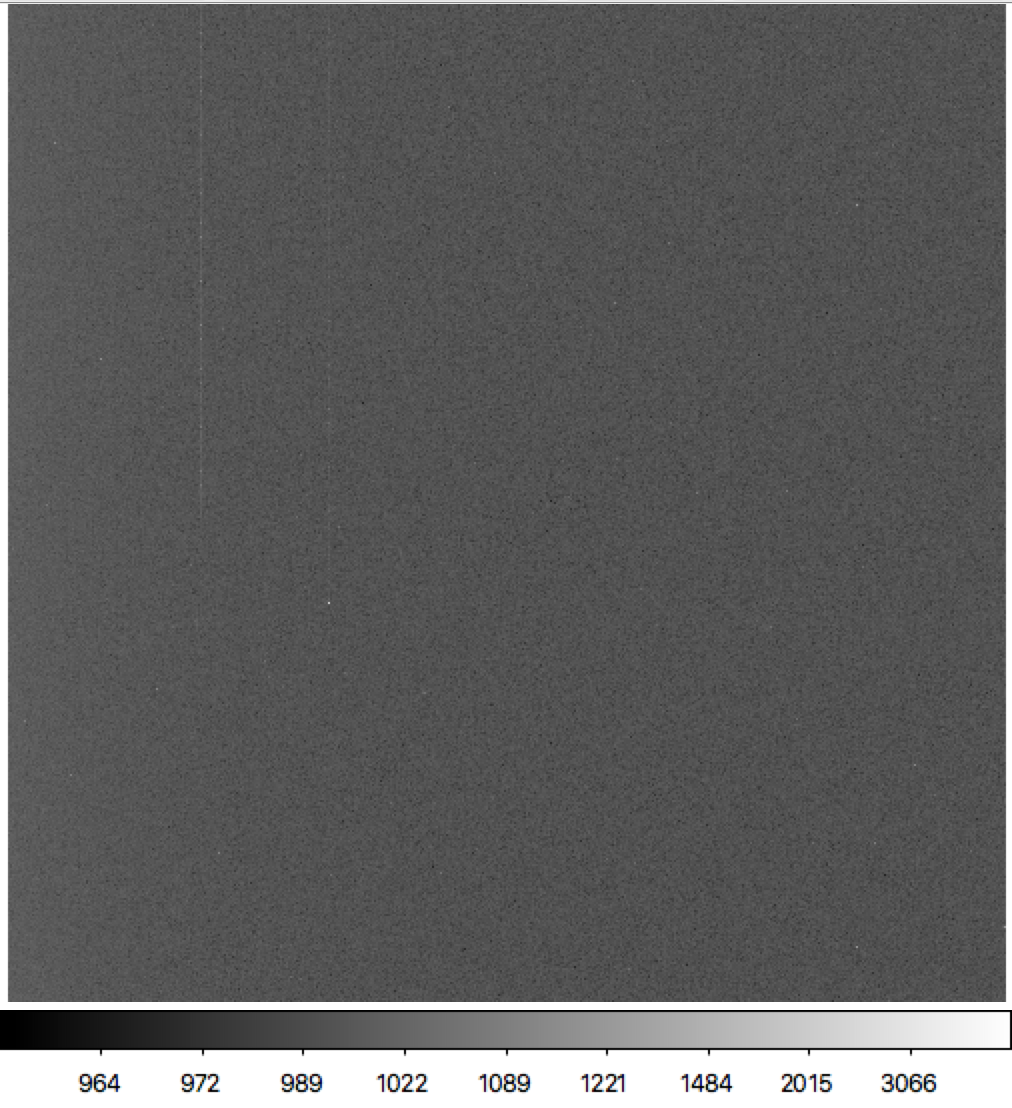
\includegraphics[width=3.5in]{../images/3p1_m10_00000000_BIAS.png}
            \caption{Bias frame}
          \label{fig:m10BIASfits}
        \end{figure}
        \begin{figure}
          \centering
            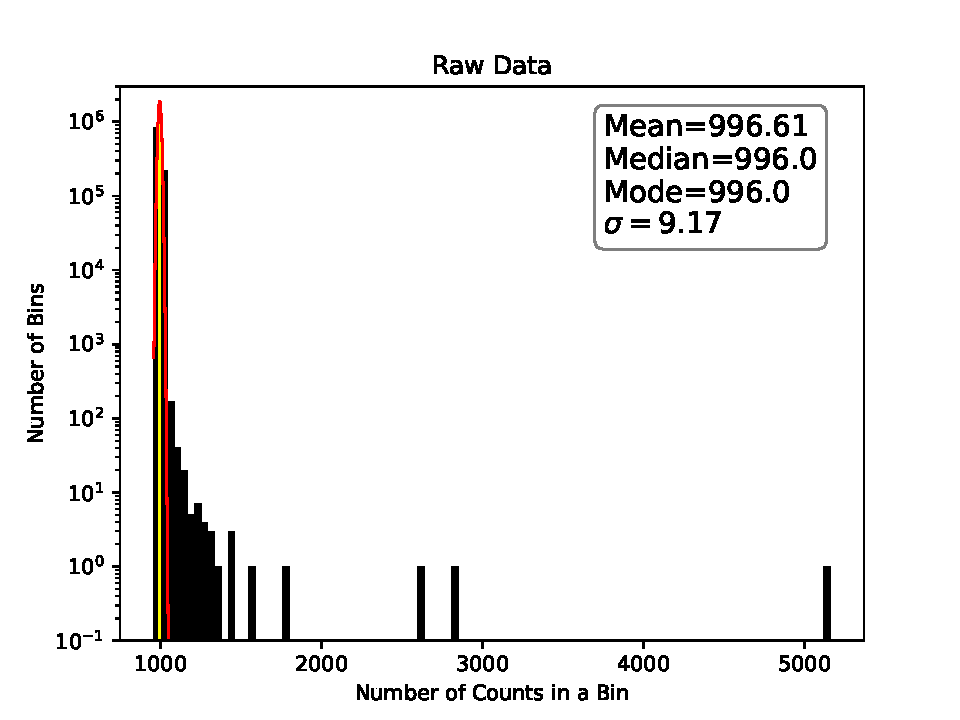
\includegraphics[width=3.5in]{../images/neg10BIAS_raw.pdf}
            \caption{}
          \label{fig:neg10BIAShisto}
        \end{figure}
        \begin{figure}
          \centering
            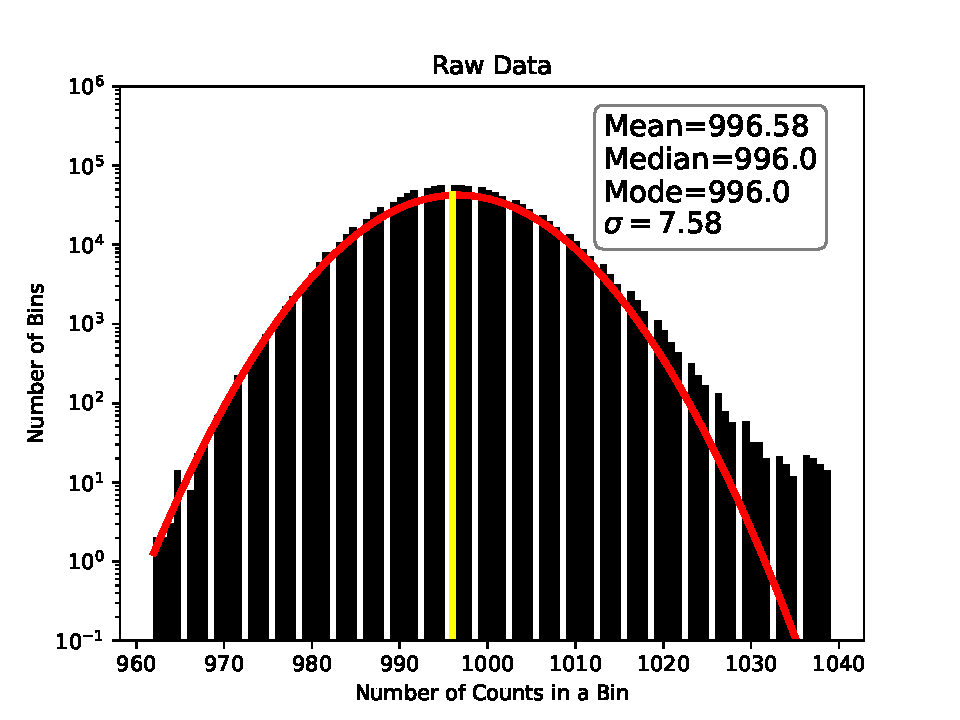
\includegraphics[width=3.5in]{../images/neg10BIAS_clipped.pdf}
            \caption{}
          \label{fig:neg10BIAShisto_clipped}
        \end{figure}
    
    %Std Dev is read noise in units of counts. Convert it to electrons.
    %Gain of the CCD camera from header is in units of electrons. 
    %Are the above consistent?
    
    %Master bias - average of 10 bias frames. Report mean and std dev
        \begin{figure}
          \centering
            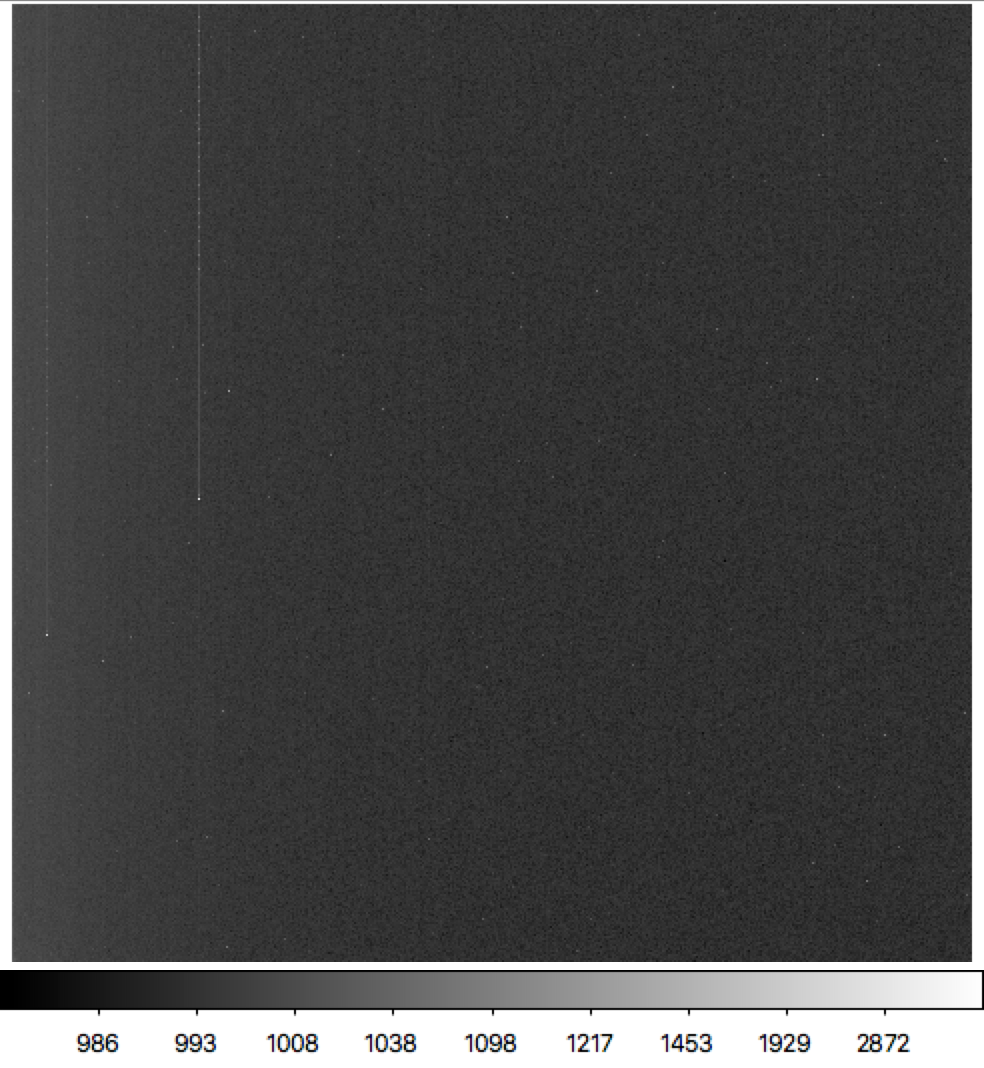
\includegraphics[width=3.5in]{../images/neg10BIAS_master.png}
            \caption{}
          \label{fig:neg10BIAS_master}
        \end{figure}
    %Report if STD Dev decreased by 1/sqrt(10)
    
    MacBook-Pro-3:Lab0 abigailbishop python3 DataAnalysis4p1-m10.py 
    Gain =  2.06
    Unclipped Read Noise:  18.884857898803837
    Clipped Read Noise:  15.618166364038043
    Percent Rejected = 0.02956390380859375
    Master mean =  994.6683856964112
    Master Standard Deviation =  6.003172702060524
    STD Decreased by:  0.3451613015828955
    1/sqrt(N\_images) =  0.31622776601683794
    
    
    %For the +10 Bias frames: 
    
        \begin{figure}
          \centering
            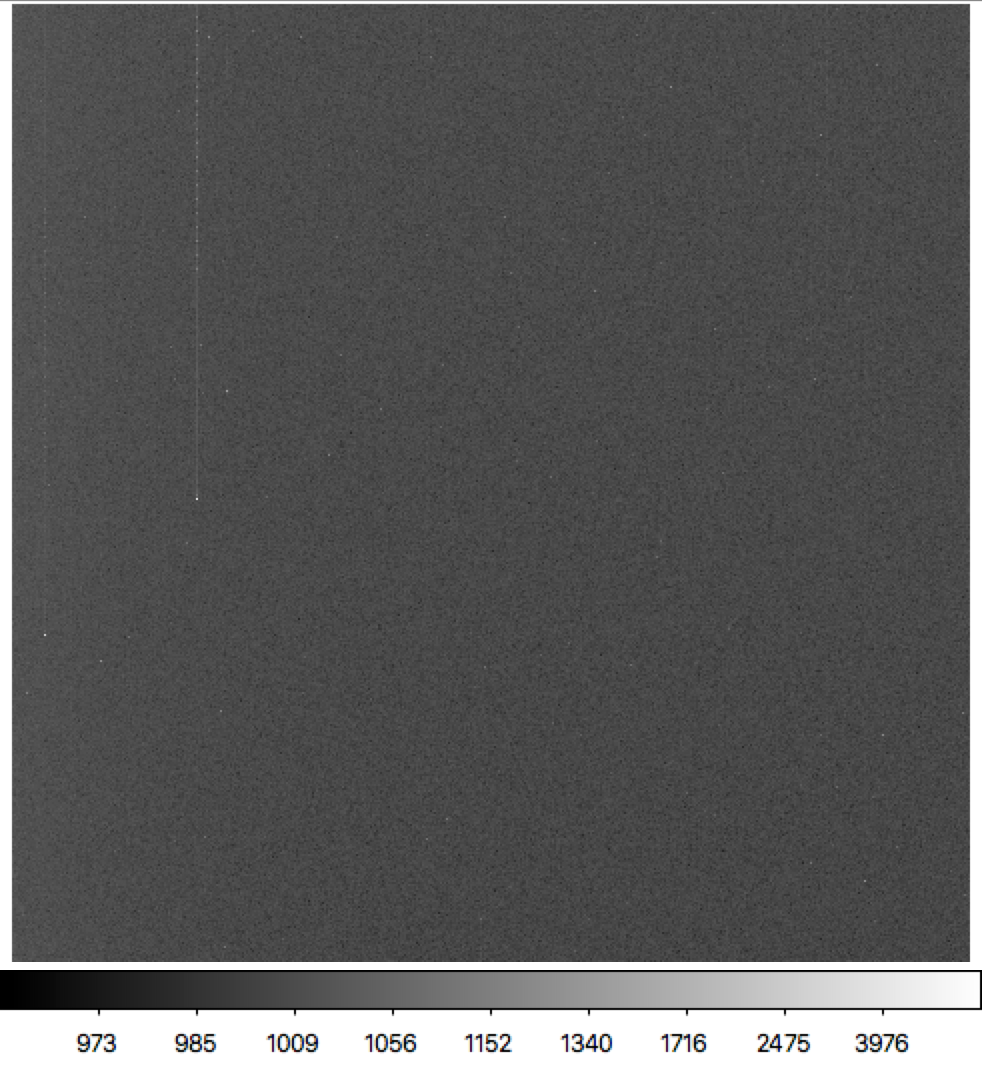
\includegraphics[width=3.5in]{../images/3p1_p10_00000000_BIAS.png}
            \caption{}
          \label{fig:p10BIASfits}
        \end{figure}
        \begin{figure}
          \centering
            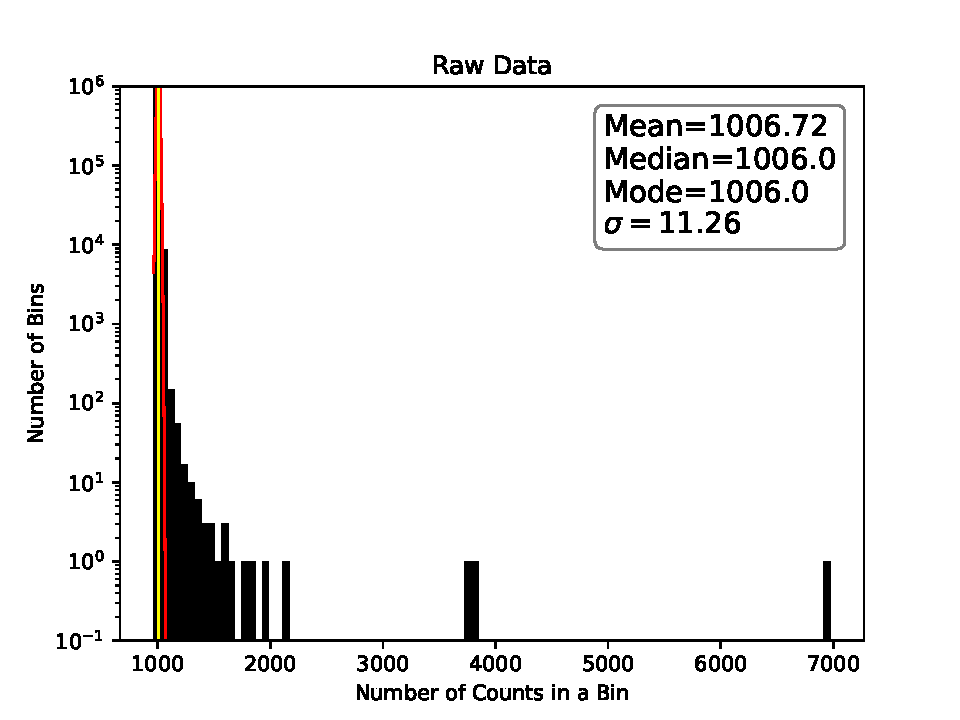
\includegraphics[width=3.5in]{../images/pos10BIAS_raw.pdf}
            \caption{}
          \label{fig:pos10BIAShisto}
        \end{figure}
    %Does the above look gaussian. Report mean, median, mode, and std dev
    %Cut rejecting the non gaussians. Fraction of pixels that gets rejected
        \begin{figure}
          \centering
            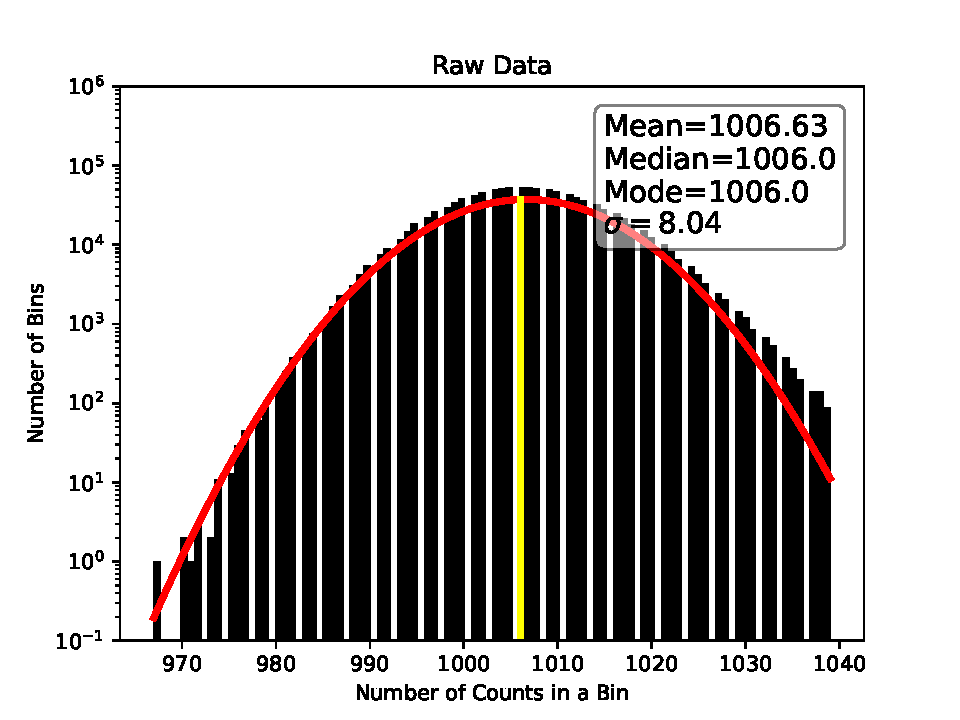
\includegraphics[width=3.5in]{../images/pos10BIAS_clipped.pdf}
            \caption{}
          \label{fig:pos10BIAShisto_clipped}
        \end{figure}
    %Does the fraction of outlier pixels change
    
    %Std Dev is read noise in units of counts. Convert it to electrons.
    %Gain of the CCD camera from header is in units of electrons. 
    %Are the above consistent?
    %Does this change from the -10 frames
    
    %Master bias - average of 10 bias frames. Report mean and std dev
        \begin{figure}
          \centering
            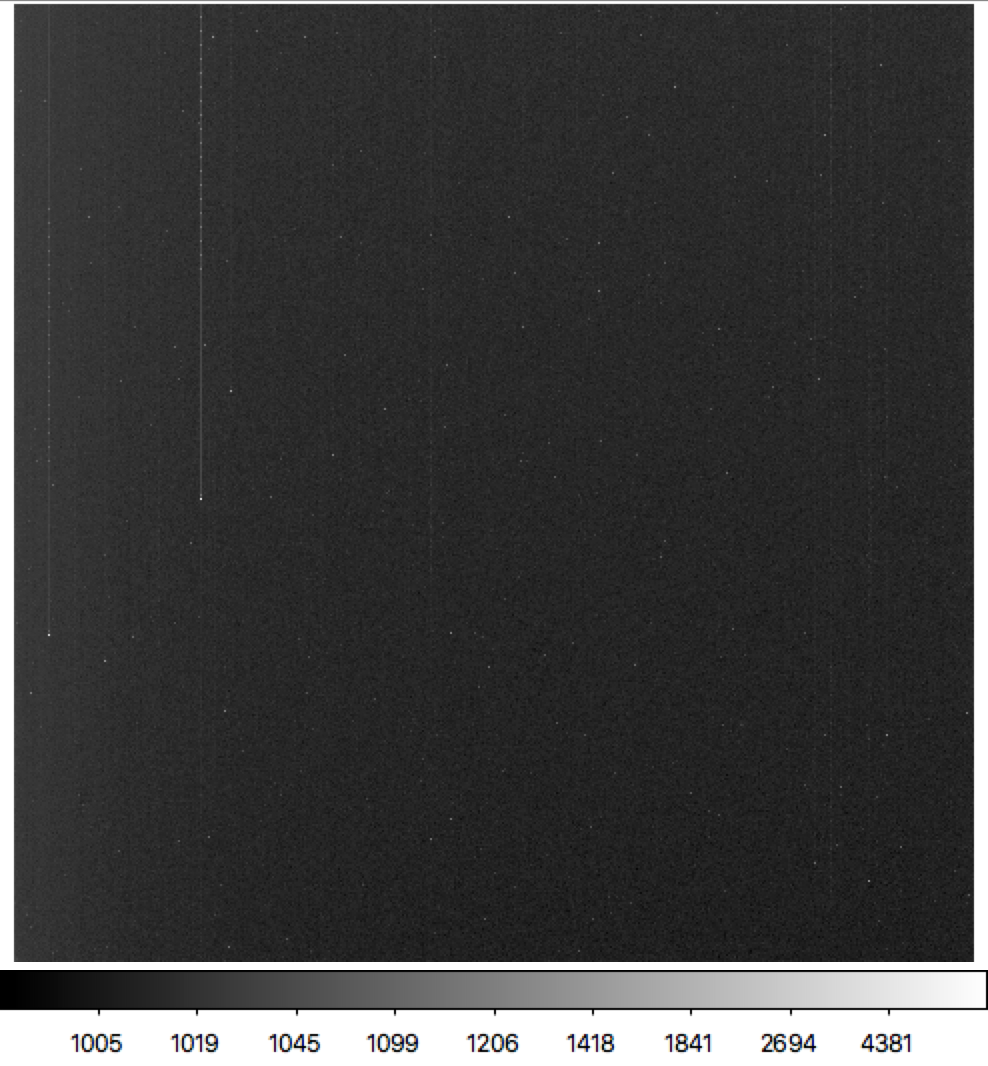
\includegraphics[width=3.5in]{../images/pos10BIAS_master.png}
            \caption{}
          \label{fig:pos10BIAS_master}
        \end{figure}
    %Report if STD Dev decreased by 1/sqrt(10)
    
    MacBook-Pro-3:Lab0 abigailbishop python DataAnalysis4p1-p10.py 
    Gain =  2.06
    Unclipped Read Noise:  23.186913206437666
    Clipped Read Noise:  16.555773015334577
    Percent Rejected = 0.09555816650390625
    Master mean =  1013.5294130325318
    Master Standard Deviation =  10.1260447421899
    STD Decreased by:  0.10036959283050784
    1/sqrt{N\_images} =  0.31622776601683794
    
  \subsection{Analysis of Dark Frames}
  
    %For the -10 C Dark frames 
    
        \begin{figure}
          \centering
            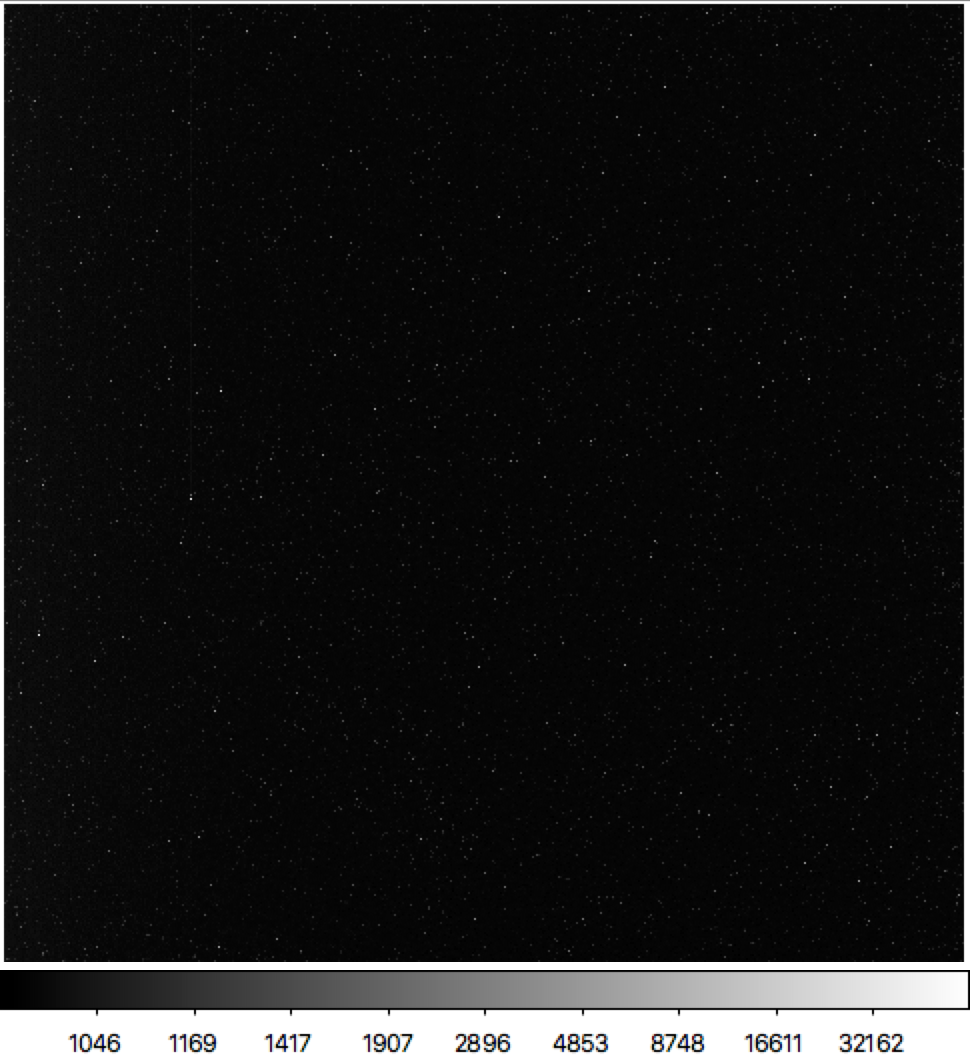
\includegraphics[width=3.5in]{../images/neg10dark_adjusted.png}
            \caption{}
          \label{fig:m10DARKfits}
        \end{figure}
        \begin{figure}
          \centering
            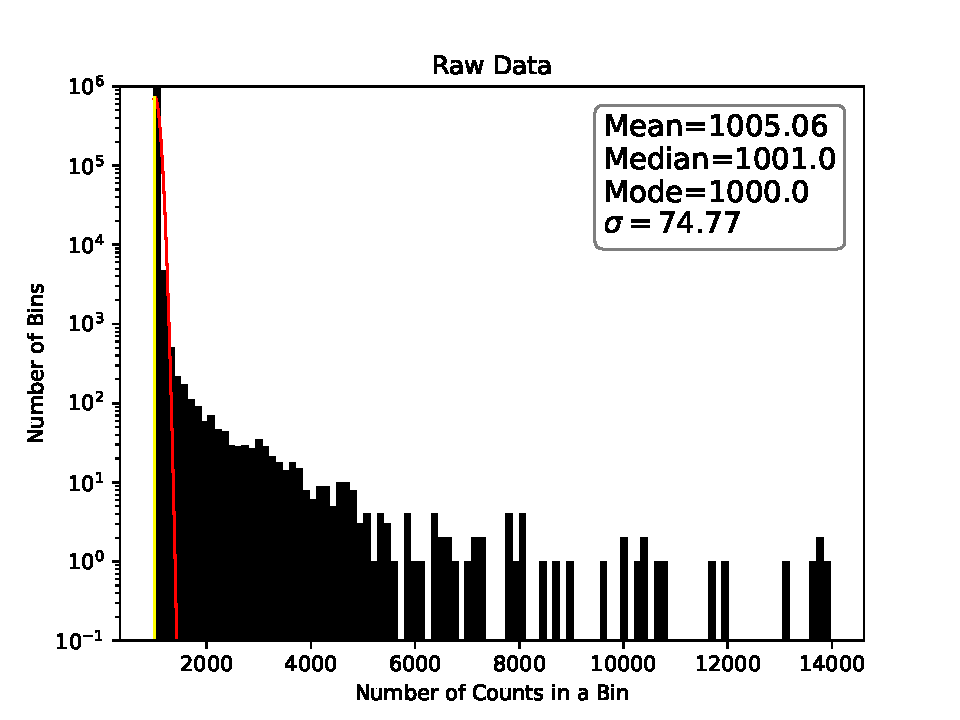
\includegraphics[width=3.5in]{../images/neg10DARK_noOutliers.pdf}
            \caption{}
          \label{fig:neg10DARKhisto}
        \end{figure}
    %Does it look Gaussian? report mean, mode, median, stddev
    %Cut selecting pixels following gaussian dist. report mean, median, mode, std dev
        \begin{figure}
          \centering
            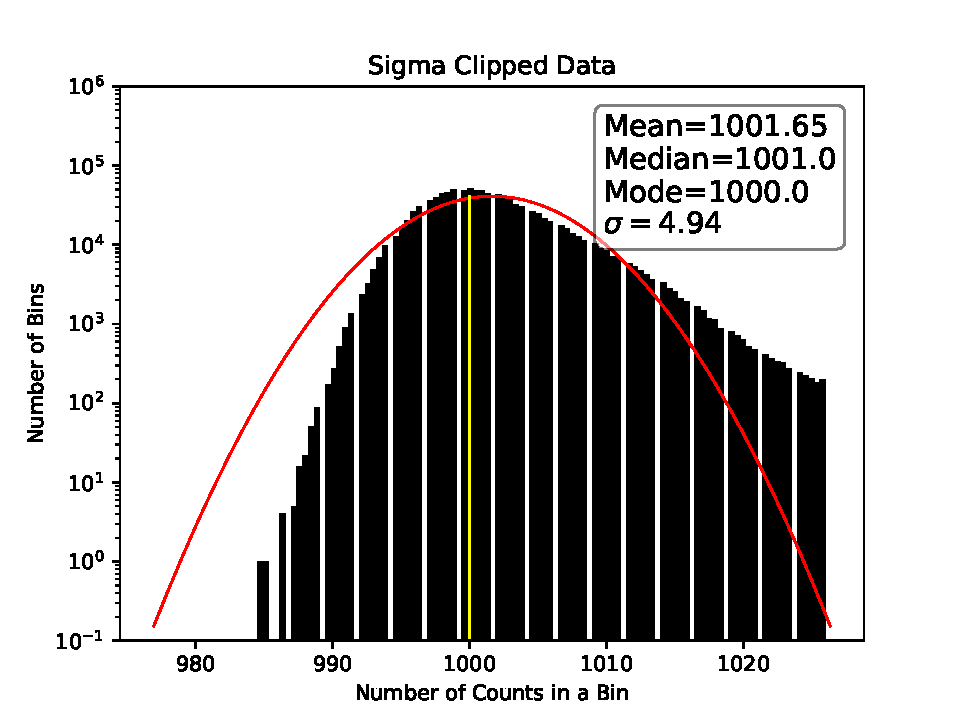
\includegraphics[width=3.5in]{../images/neg10DARK_cut.pdf}
            \caption{}
          \label{fig:neg10DARK_cut}
        \end{figure}
    %percent of pixels rejected. 
    %How do mean, median, mode, and std dev change? Which do not change?
    %How do you identify hot pixels? What fraction are hot. 
    
    %Subtract master bias and quantify typical counts and the uncertainty. Justify your choices
        \begin{figure}
          \centering
            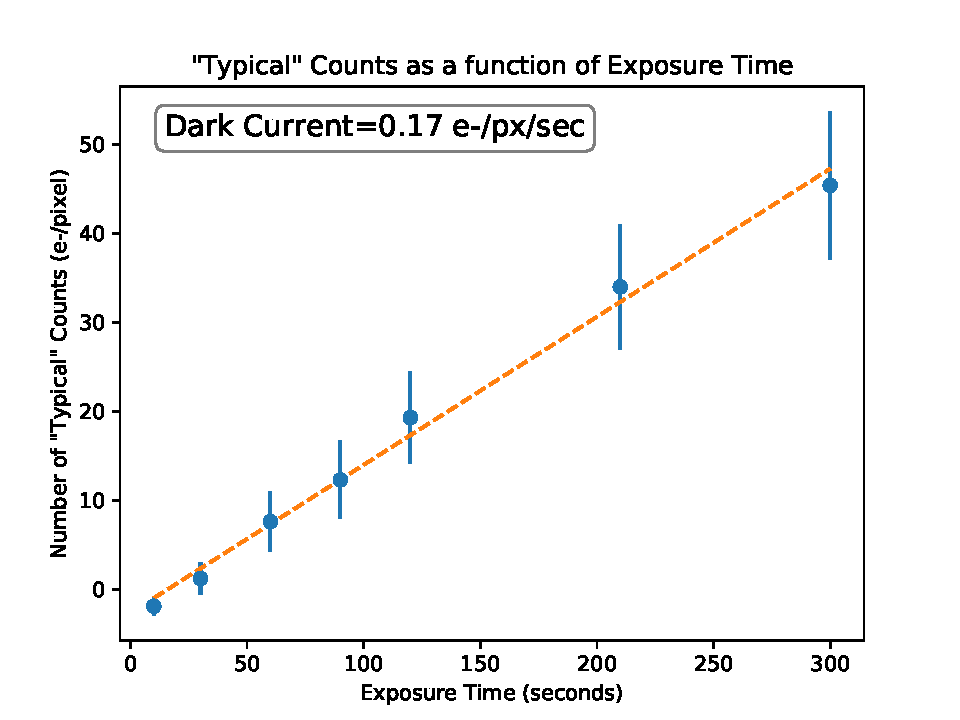
\includegraphics[width=3.5in]{../images/neg10DARK_typical-exposure.pdf}
            \caption{}
          \label{fig:neg10DARK_typical-exposure}
        \end{figure}
    %linear regression. What is the dark current?
    
    python DataAnalysis4p2-m10.py 
    Percent Rejected = 1.7302694635048852
    Percent Hot = 1.7951011657714844
    
    %For the +10 C Dark frames 
    
        \begin{figure}
          \centering
            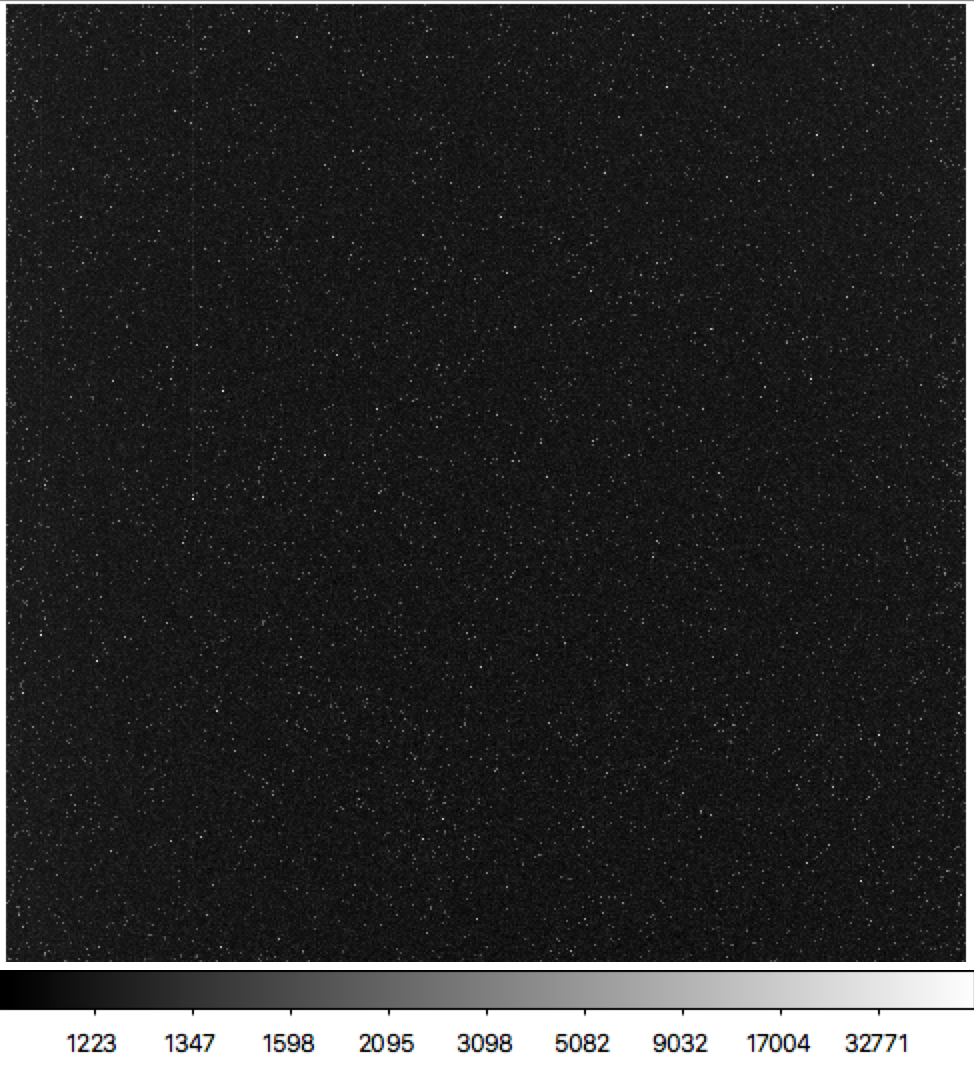
\includegraphics[width=3.5in]{../images/pos10dark_adjusted.png}
            \caption{}
          \label{fig:p10DARKfits}
        \end{figure}
        \begin{figure}
          \centering
            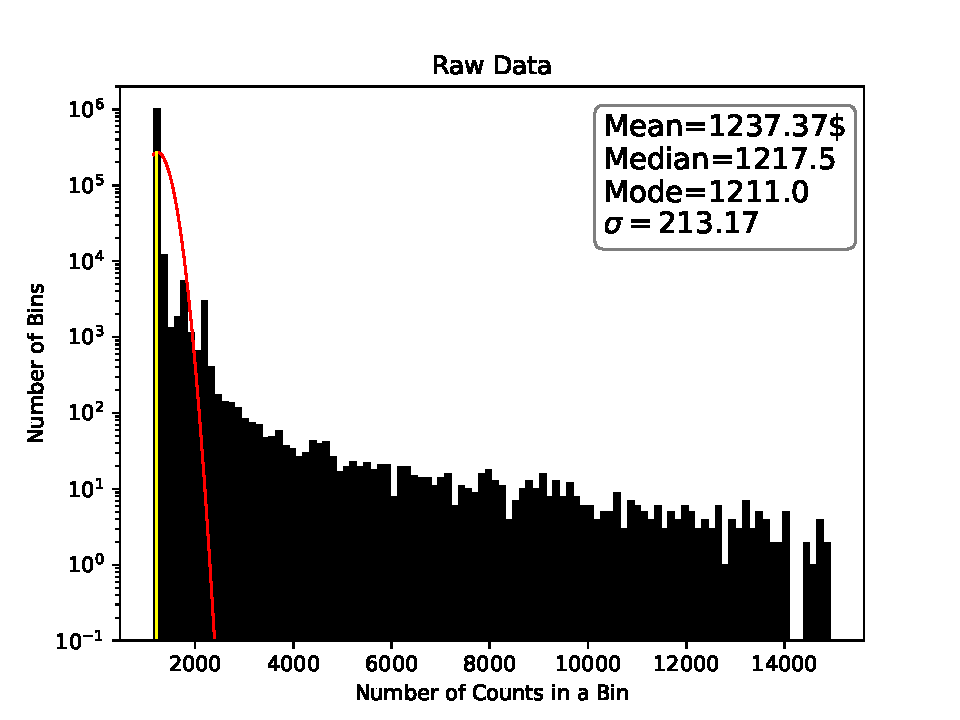
\includegraphics[width=3.5in]{../images/pos10DARK_noOutliers.pdf}
            \caption{}
          \label{fig:pos10DARKhisto}
        \end{figure}
    %Does it look Gaussian? report mean, mode, median, stddev
    %Cut selecting pixels following gaussian dist. report mean, median, mode, std dev
        \begin{figure}
          \centering
            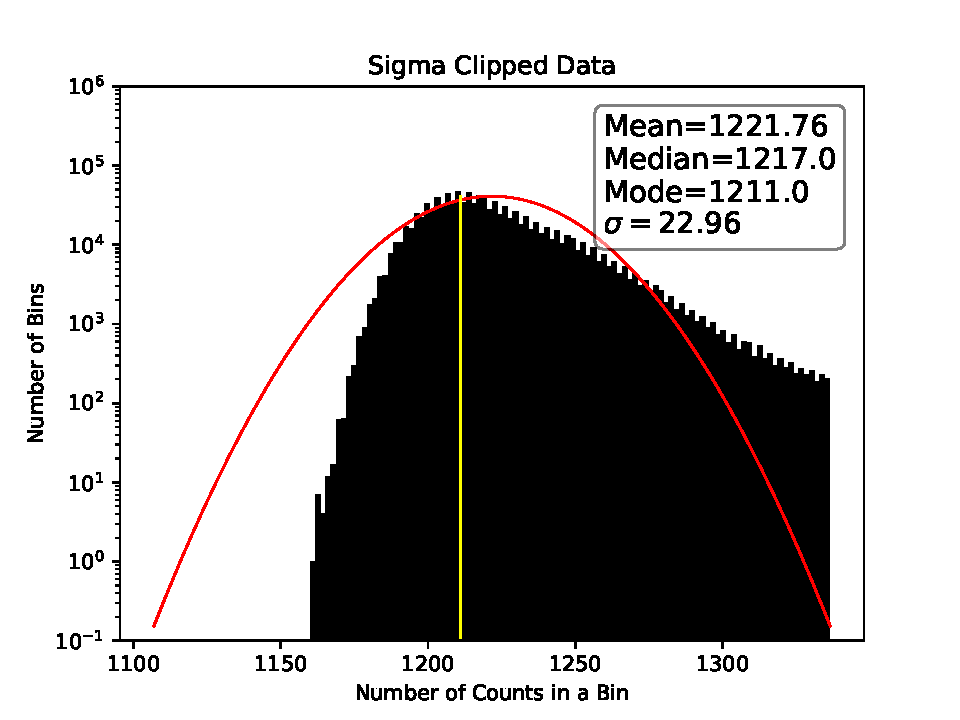
\includegraphics[width=3.5in]{../images/pos10DARK_cut.pdf}
            \caption{}
          \label{fig:pos10DARK_cut}
        \end{figure}
    %percent of pixels rejected. 
    %How do mean, median, mode, and std dev change? Which do not change?
    %How do you identify hot pixels? What fraction are hot. 
    %Does the fraction of hot pixels change from before?
    
    %Subtract master bias and quantify typical counts and the uncertainty. Justify your choices
        \begin{figure}
          \centering
            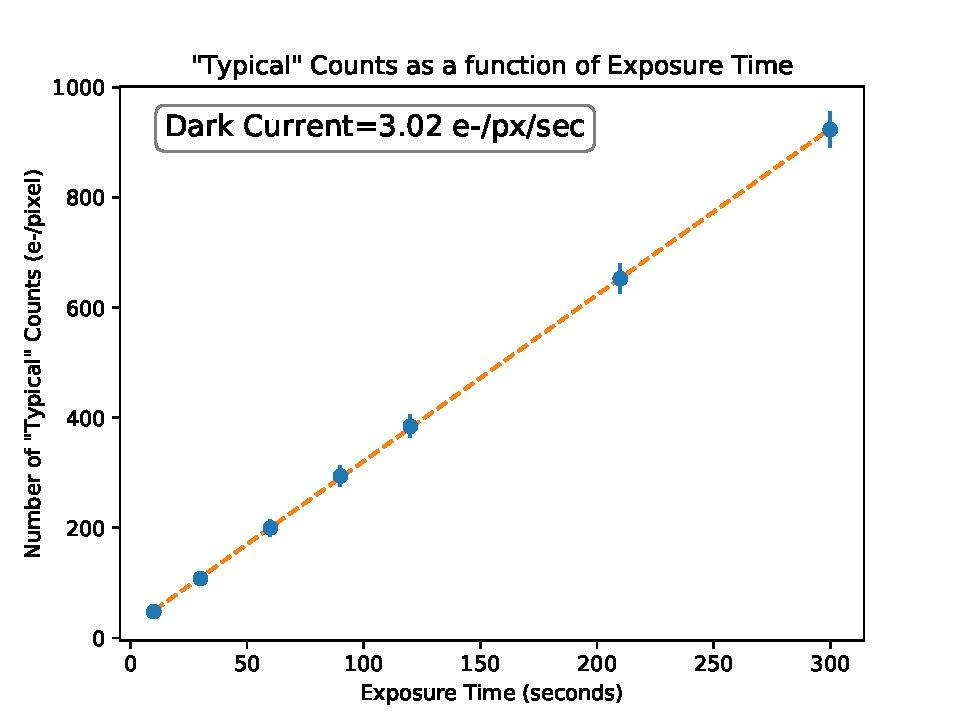
\includegraphics[width=3.5in]{../images/pos10DARK_typical-exposure.pdf}
            \caption{}
          \label{fig:pos10DARK_typical-exposure}
        \end{figure} 
    %linear regression. What is the dark current?
    %How does the dark current change?
    
    python DataAnalysis4p2-p10.py 
    Percent Rejected = 1.8139990481250066
    Percent Hot = 1.8419265747070312
    
  \subsection{Analysis of Flat Fields}
    
        \begin{figure}
          \centering
            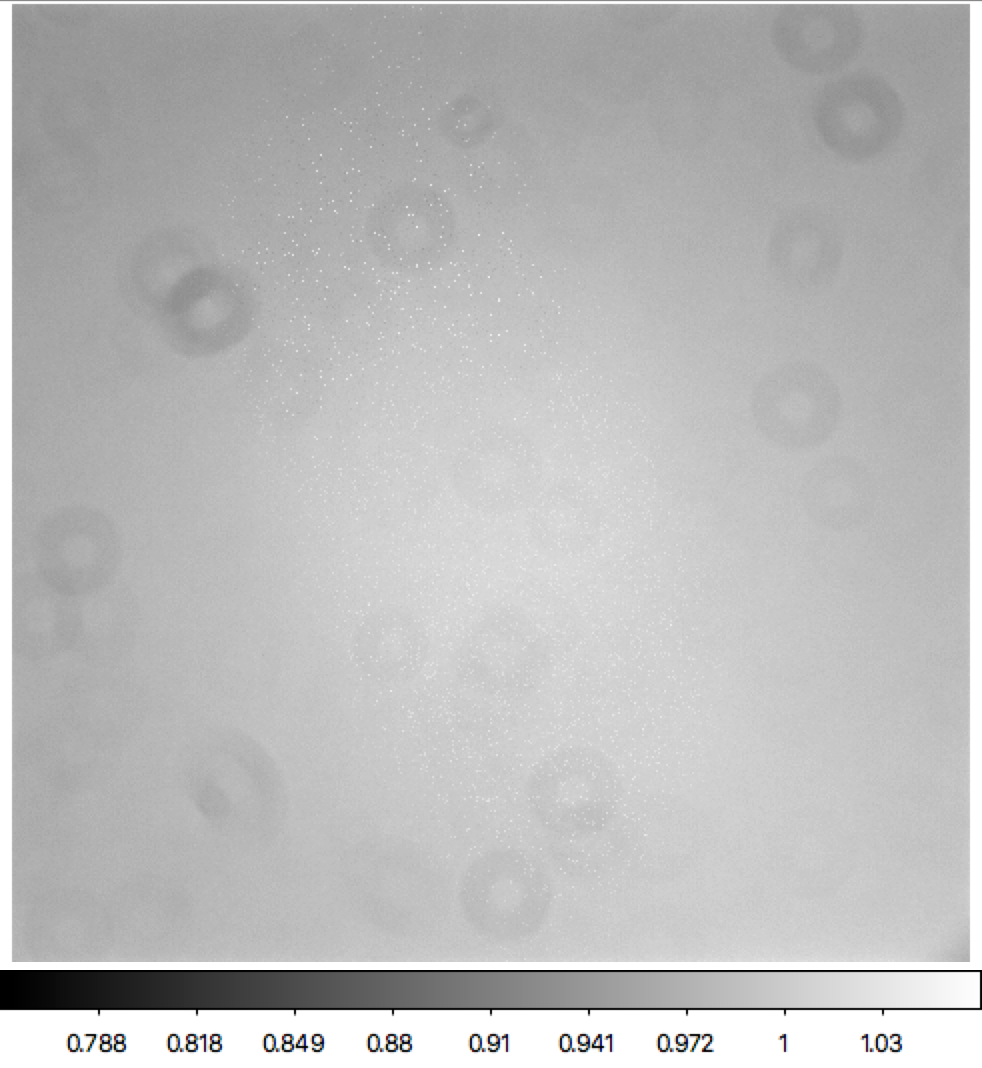
\includegraphics[width=3.5in]{../images/flat_master.png}
            \caption{}
          \label{fig:flat_master}
        \end{figure}
    
    %Identify regions of particularly low count rates. 
    %Quantify what fraction of light is received as pixels move farther from the center
    
        \begin{figure}
          \centering
            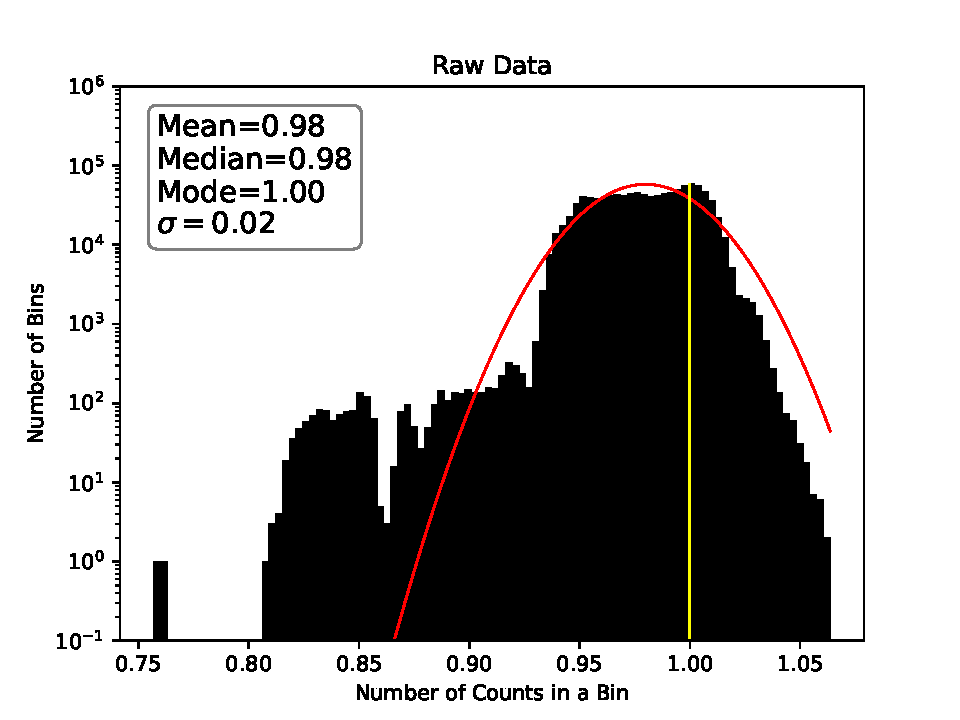
\includegraphics[width=3.5in]{../images/flat_master_raw.pdf}
            \caption{}
          \label{fig:flat_masterhisto}
        \end{figure}
    %Identify dead pixels
    %Perhaps a note on the elliptical trend relating to not being cool enough.
    
        \begin{figure}
          \centering
            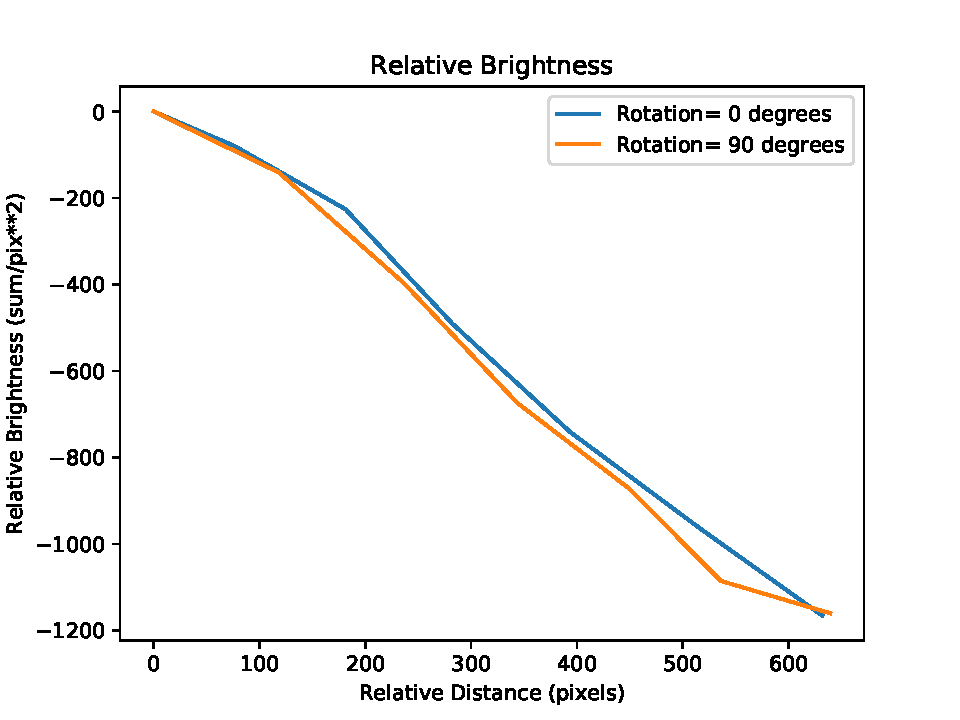
\includegraphics[width=3.5in]{../images/brightness-distance.pdf}
            \caption{}
          \label{fig:brightness-distance}
        \end{figure}
    %How would the 'observed' magnitude of a star change if it was in the center as opposed to the outside of the CCD?
    
        \begin{figure}
          \centering
            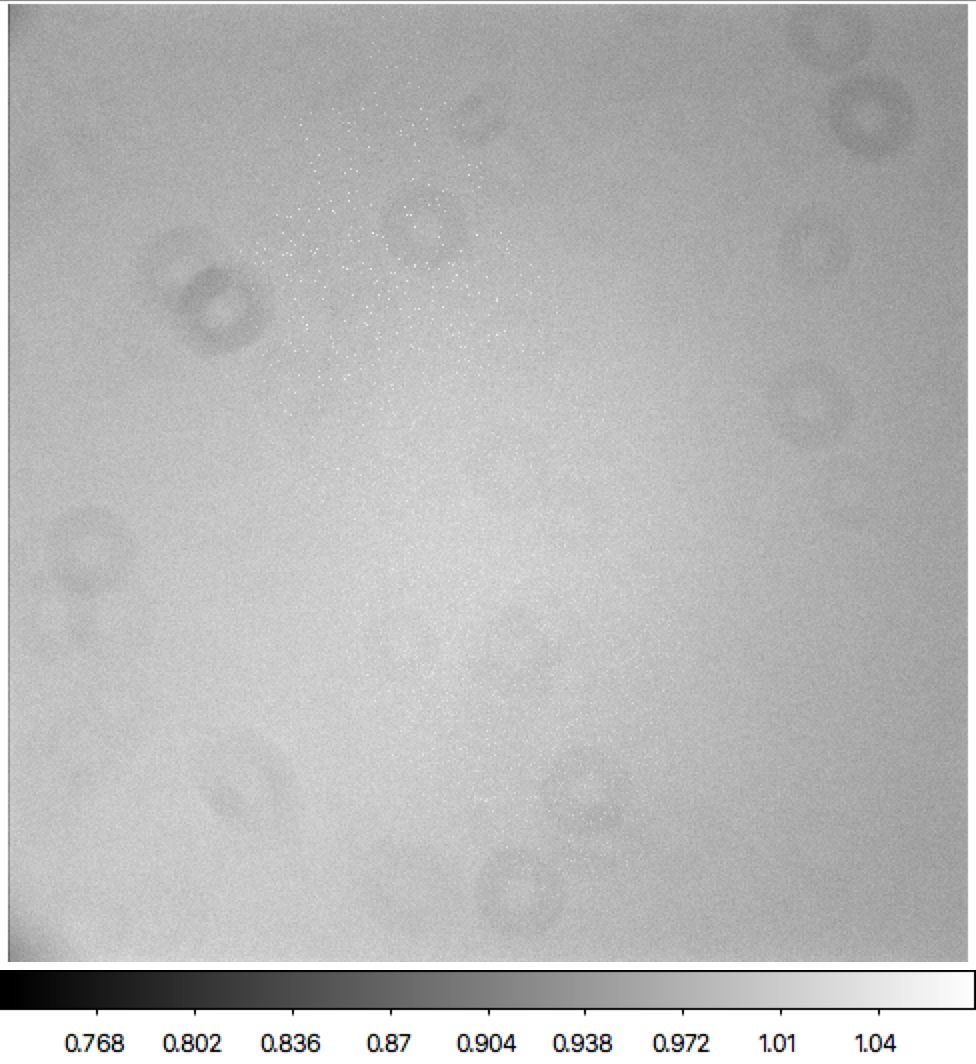
\includegraphics[width=3.5in]{../images/flat_master_r90.png}
            \caption{}
          \label{fig:flat_master-r90}
        \end{figure}
        \begin{figure}
          \centering
            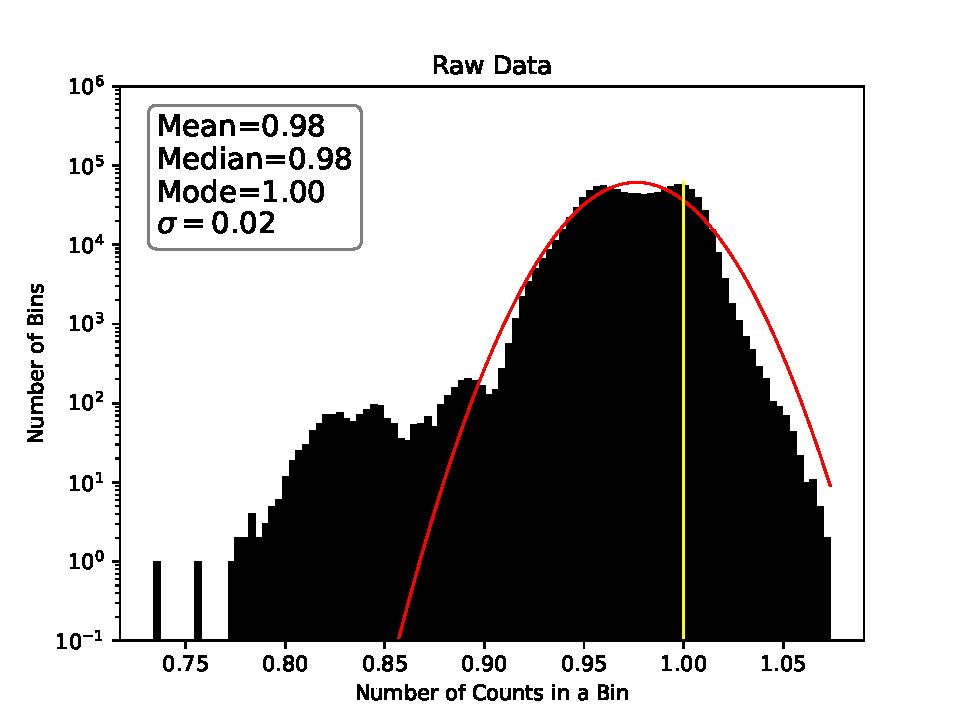
\includegraphics[width=3.5in]{../images/flat_master_raw_r90.pdf}
            \caption{}
          \label{fig:flat_masterhisto_r90}
        \end{figure}
    %How does the flat change. 
    %If you forgot to take flats on the night of observations, can you retake them later?
    
  \subsection{Bad Pixel Map}
  
        \begin{figure}
          \centering
            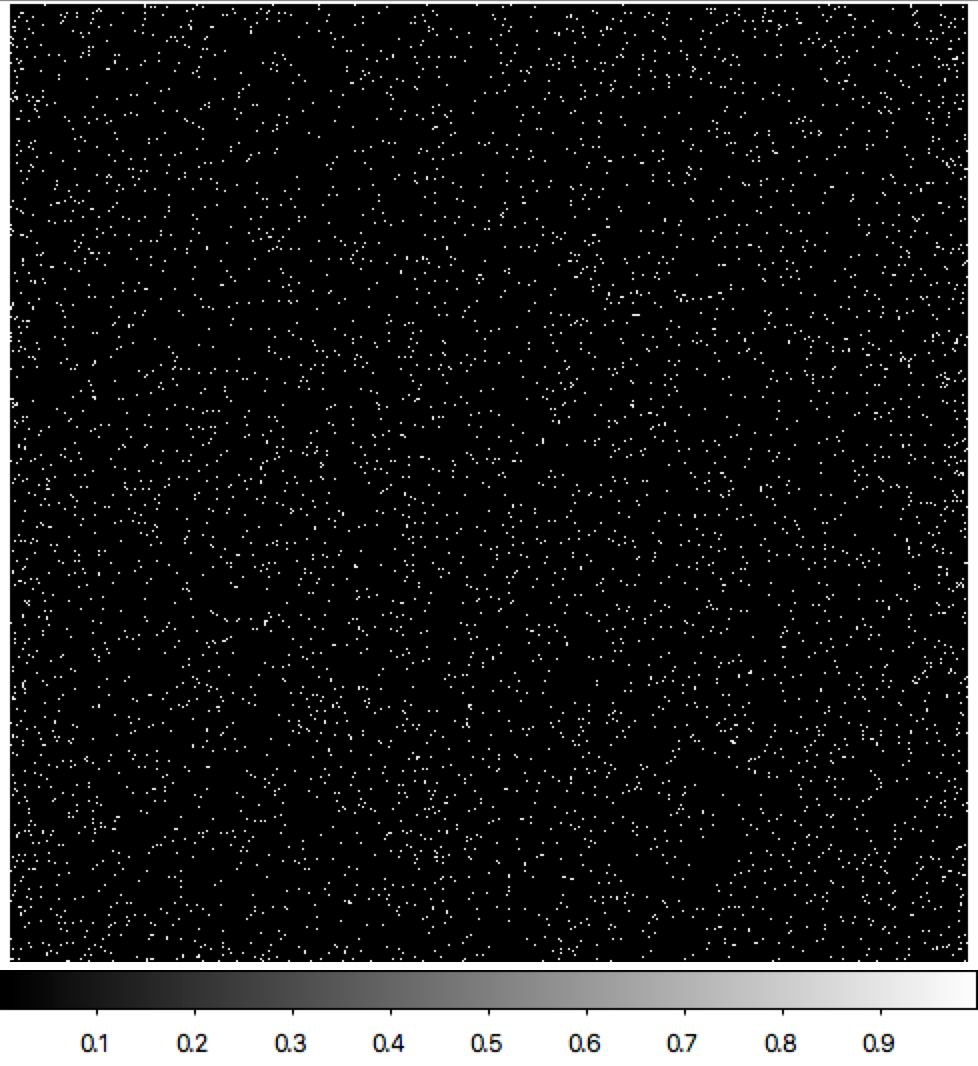
\includegraphics[width=3.5in]{../images/bad_pixel_map.png}
            \caption{}
          \label{fig:bad_pixel_map}
        \end{figure}
    
  \subsection{Analysis of Spectroscopy}
  
        \begin{figure}
          \centering
            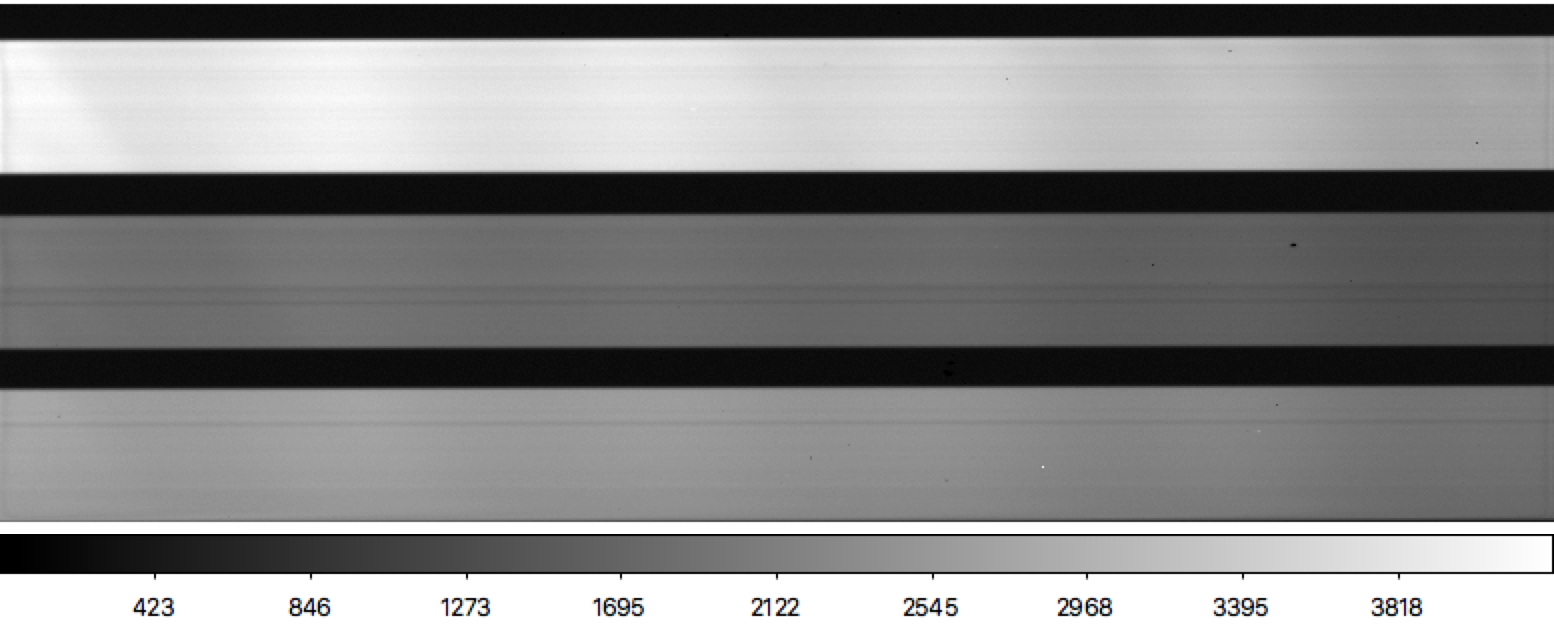
\includegraphics[width=3.5in]{../images/master_DomeFlat.png}
            \caption{}
          \label{fig:master_DomeFlat}
        \end{figure}
    
    %Which line on the master flat is the 50 micrometer slit?
    
        \begin{figure}
          \centering
            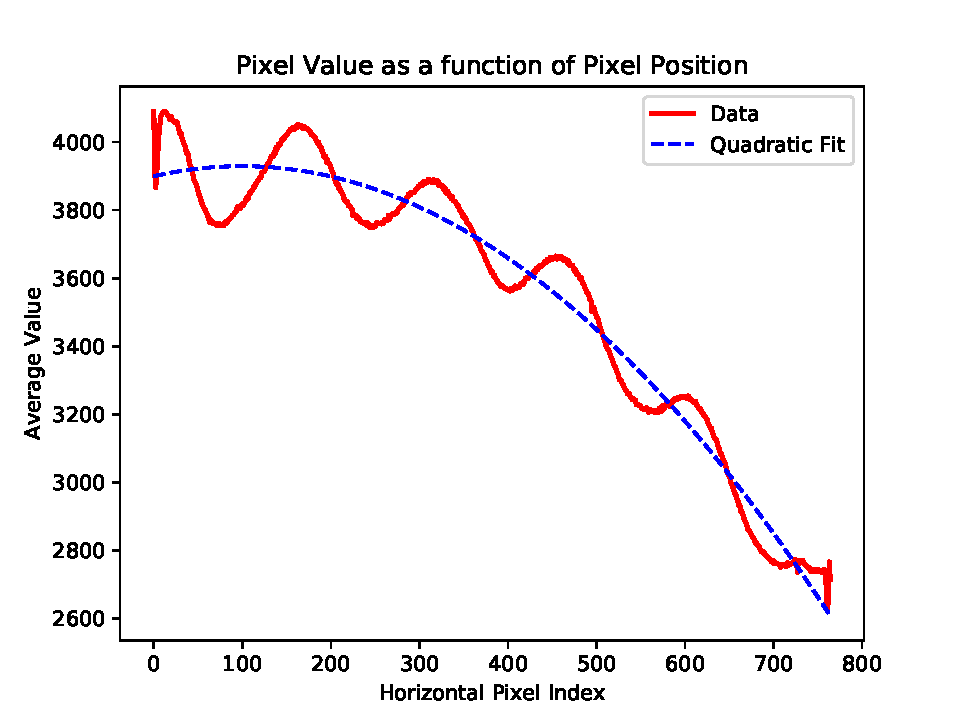
\includegraphics[width=3.5in]{../images/spectrograph_crop_fit.pdf}
            \caption{}
          \label{fig:spectrograph_crop_fit}
        \end{figure}
    
        \begin{figure}
          \centering
            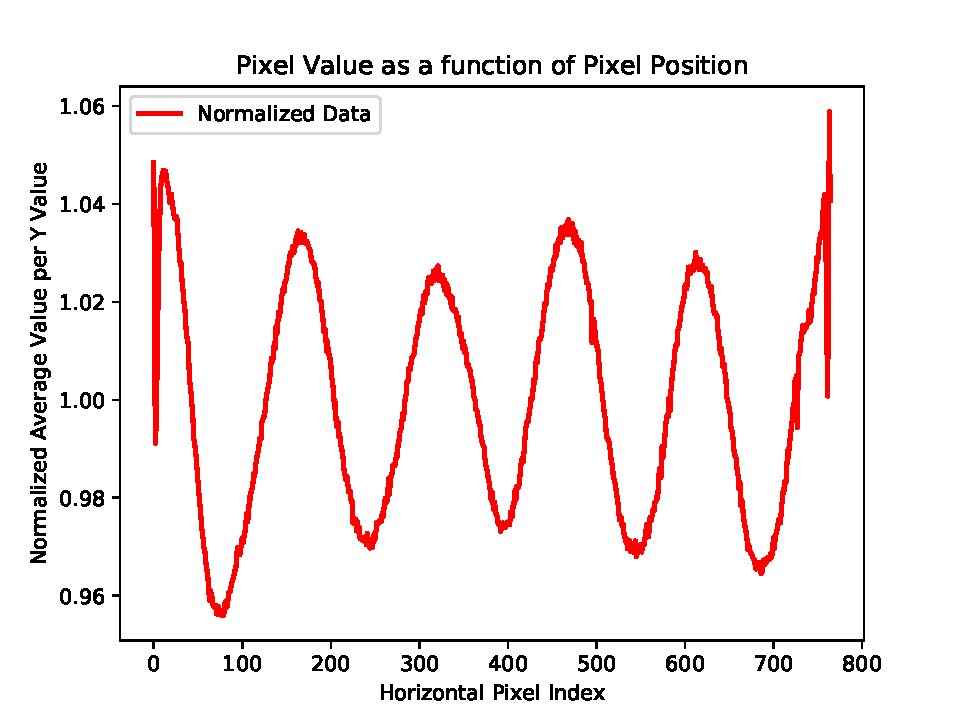
\includegraphics[width=3.5in]{../images/spectrograph_cropnorm_fit.pdf}
            \caption{}
          \label{fig:spectrograph_cropnorm_fit}
        \end{figure}
    
        \begin{figure}
          \centering
            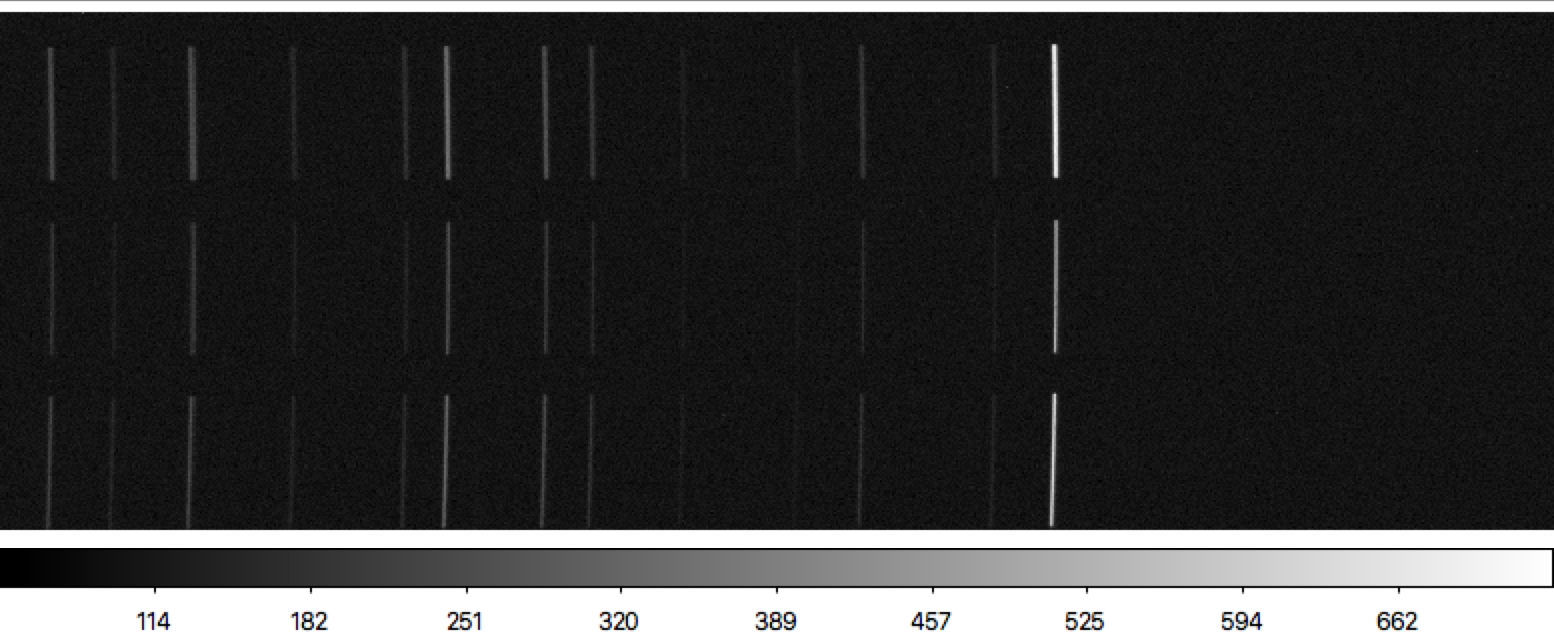
\includegraphics[width=3.5in]{../images/masterflat_lamp.png}
            \caption{}
          \label{fig:masterflat_lamp}
        \end{figure}
        \begin{figure}
          \centering
            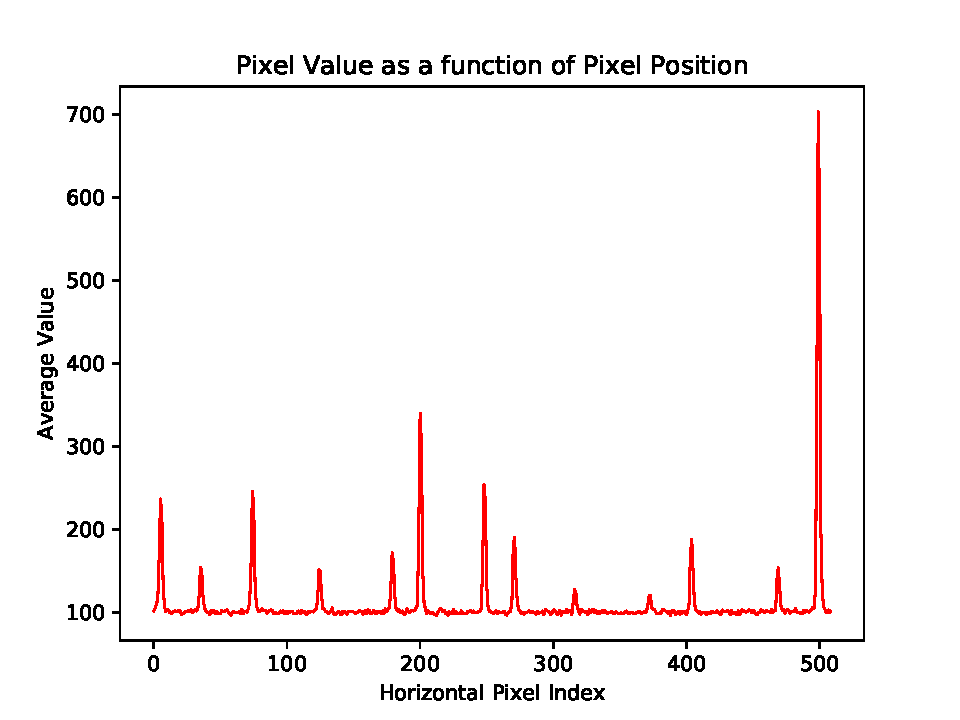
\includegraphics[width=3.5in]{../images/spectrograph_crop_values-Lamp.pdf}
            \caption{}
          \label{fig:spectrograph_crop_values-Lamp}
        \end{figure}
        \begin{figure}
          \centering
            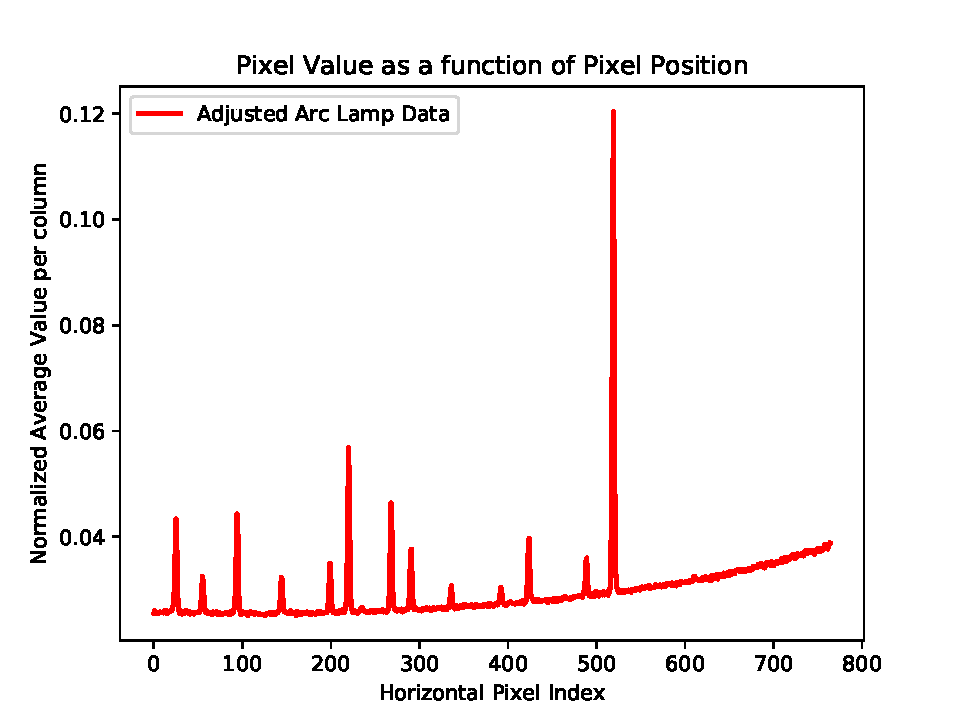
\includegraphics[width=3.5in]{../images/spectrograph_lampadj_fit.pdf}
            \caption{}
          \label{fig:spectrograph_lampadj_fit}
        \end{figure}
    
    %Wavelength vs pixel position and best fit line. 
    
    %Dispersion of spectrograph. 
    %Length of spectrum in angstroms covered by our spectrograph
    %Arc lamp spectrum vs wavelength (not pixel) with labels of neon
    

\section{Results and Conclusion}


\end{document}  